%+210 to left and -210 to right if I want to move one subfigure.

\begin{figure}[!h]
%\vspace{-1pt} %takes away some white space before figure
\centering
\begin{subfigure}[b]{1.0\textwidth}
\centering
	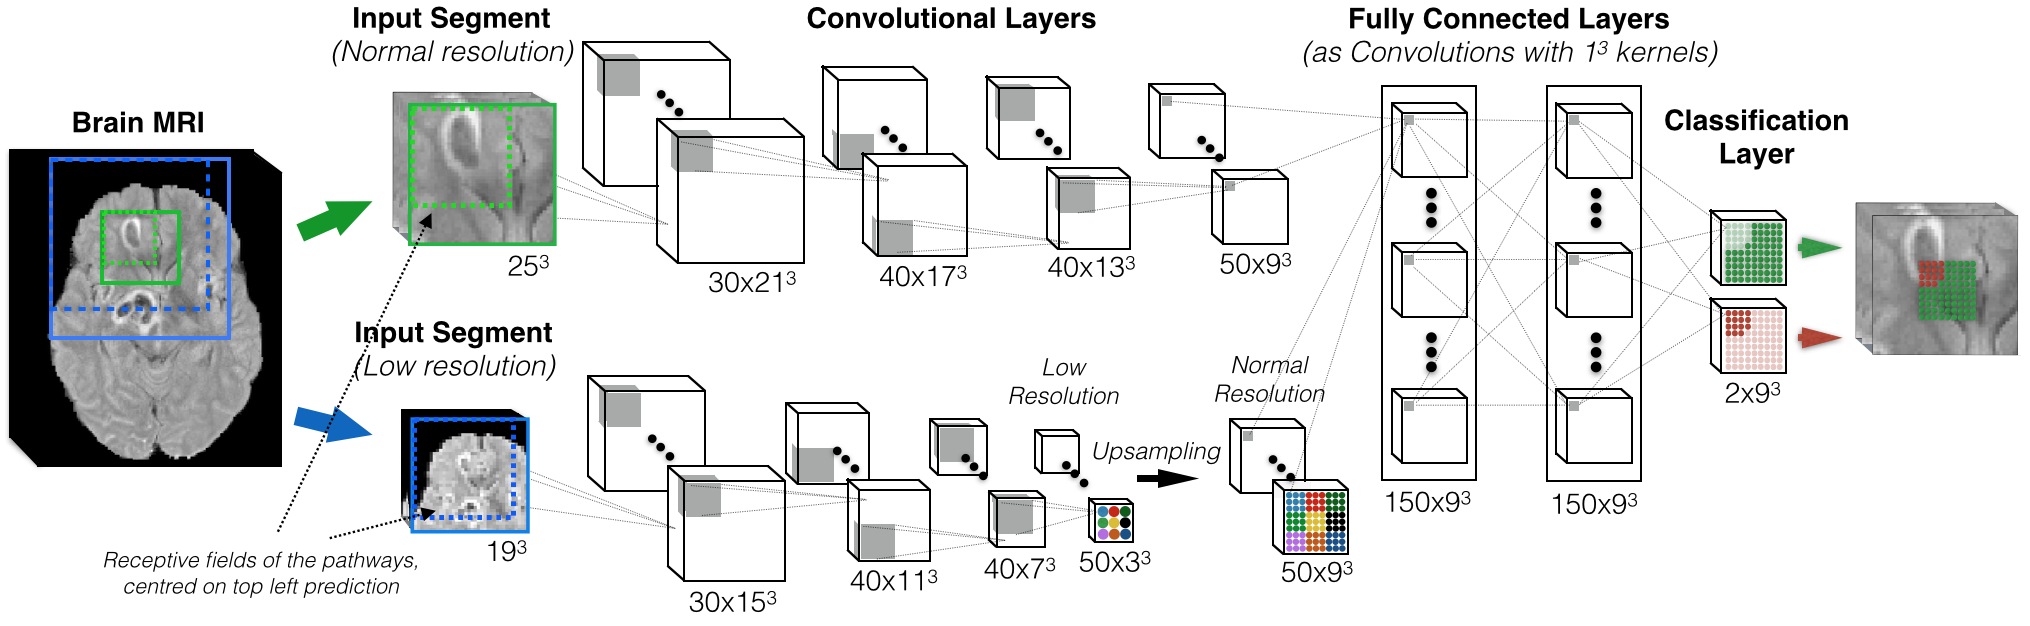
\includegraphics[clip=true, trim=0pt 0pt 0pt 0pt, width=1.0\textwidth]{figures/methodSection/multiscale/cnnSystemMultiscale.png}
\end{subfigure}
\caption{Multi-scale 3D CNN with two convolutional pathways. The kernels of the two pathways are here of size $5^3$ (for illustration only to reduce the number of layers in the figure). The neurons of the last layers of the two pathways thus have receptive fields of size $17^3$ voxels. The inputs of the two pathways are centered at the same image location, but the second segment is extracted from a down-sampled version of the image by a factor of 3. The second pathway processes context in an actual area of size $51^3$ voxels. \textit{DeepMedic}, our proposed 11-layers architecture, results by replacing each layer of the depicted pathways with two that use $3^3$ kernels (see Sec.~\ref{subsec:buildingADeeperNetwork}). Number of FMs and their size depicted as (\textit{Number $\times$ Size}).}
\label{fig:cnnMultiscale}
\end{figure}
%\vspace{-1pt} %takes away some white space before figure